\section{Appendix A}\label{sec:appA}
\begin{verbatim}
tic;
Nsteps = 80;   % Number of iterations
Nplot = 101;   % Fineness of plots
T = 10*eps;   % Time delay
az = 13;      % Plot viewing angle
el = 48;      % Plot viewing height
v = 0.0;      % Camera speed
fix_axes = 0;               % Set to 1 for fixed axes
plot_range = [-0.1 1.1];    % z-axis range if fixed
% col_range = plot_range;   % Fixed colour range
% col_range = [-.7 1.1];
col_range = 'manual';       % Varying colour range
rec = 0;                    % record on/off
xg = linspace(-1,1,Nplot);
yg = linspace(-1,1,Nplot);
[XX,YY] = meshgrid(xg,yg);
ZZ = NaN(size(XX));

[indy_up,indx_up]=find(XX>=0);
indx_up = unique(indx_up);
indy_up = unique(indy_up);

[indy_lo,indx_lo]=find(YY<=0);
indx_lo = unique(indx_lo);
indy_lo = unique(indy_lo);

indices_all=find(XX>=0|YY<=0);
ZZ(indices_all)=1;
Du_dy=(ZZ(1:Nplot-2,:)-ZZ(3:Nplot,:));
Du_dx=(ZZ(:,3:Nplot)-ZZ(:,1:Nplot-2));
diffy_ind=~isnan(Du_dy);
diffx_ind=~isnan(Du_dx);
\end{verbatim}


\subsection*{Export geometry}

\begin{verbatim}
load('upper_rectangle')
load('lower_rectangle')
\end{verbatim}


\subsection*{Define the problem}

\begin{verbatim}
a = 1;
c = 1;        % Coeffs in PDE
f = 1;        % RHS of PDE
% f = '1+x.^2+12*(y+1)';
% f = '1./(x.^2+(y+1/2).^2)-1./((x-1/2).^2+y.^2)';

initguess=@(x,y) abs(log(1./((x.^2+y.^2).^.5))).^0.4999 % u0=infinity
% initguess=@(x,y) 1;
% initguess = @(x,y) 0; % u0~=1 @(0,0)
% initguess = @(x,y) -1-sin(22*x).*sin(10*y);
% initguess = @(x,y) 1-sin(22*x).*sin(10*y);
% initguess = @(x,y) 0.0+(min(x.^2+(y+.5).^2,(x-.5).^2+y.^2)<.005);
% initguess = @(x,y) (min(x.^2+(y+.5).^2,(x-.5).^2+y.^2)>.05);
% initguess = @(x,y) -3+4*(x.^2+(y+1/2).^2>.001);
% initguess = @(x,y) 1-.001./(x.^2+(y+1/2).^2).^(1/3)-.001./((x-1/2).^2+y.^2).^(1/3);
%initguess = @(x,y) 10-7.*(abs(log(-x.^2-(y+1/2).^2))).^0.4999;
\end{verbatim}
\subsection*{Generate the mesh}

\begin{verbatim}
errvals_inf= zeros(4,Nsteps);
errvals_H1=zeros(4,Nsteps);

for Nmesh=25:25:100;
\end{verbatim}
\begin{verbatim}
meshgenfun = '1./(x.^2+y.^2)'; % function for adaptive mesh generation
[~,p_up,e_up,t_up]=adaptmesh(g_up,b_up,c,a,meshgenfun,'Ngen', Nmesh);
[~,p_lo,e_lo,t_lo]=adaptmesh(g_lo,b_lo,c,a,meshgenfun,'Ngen', Nmesh);
figure(1);
pdemesh(p_up,e_up,t_up);
xlim ([-1.5,1.5]);
axis equal;

figure(2);
pdemesh(p_lo,e_lo,t_lo);
xlim ([-1.5,1.5]);
axis equal;
\end{verbatim}

   
      
    
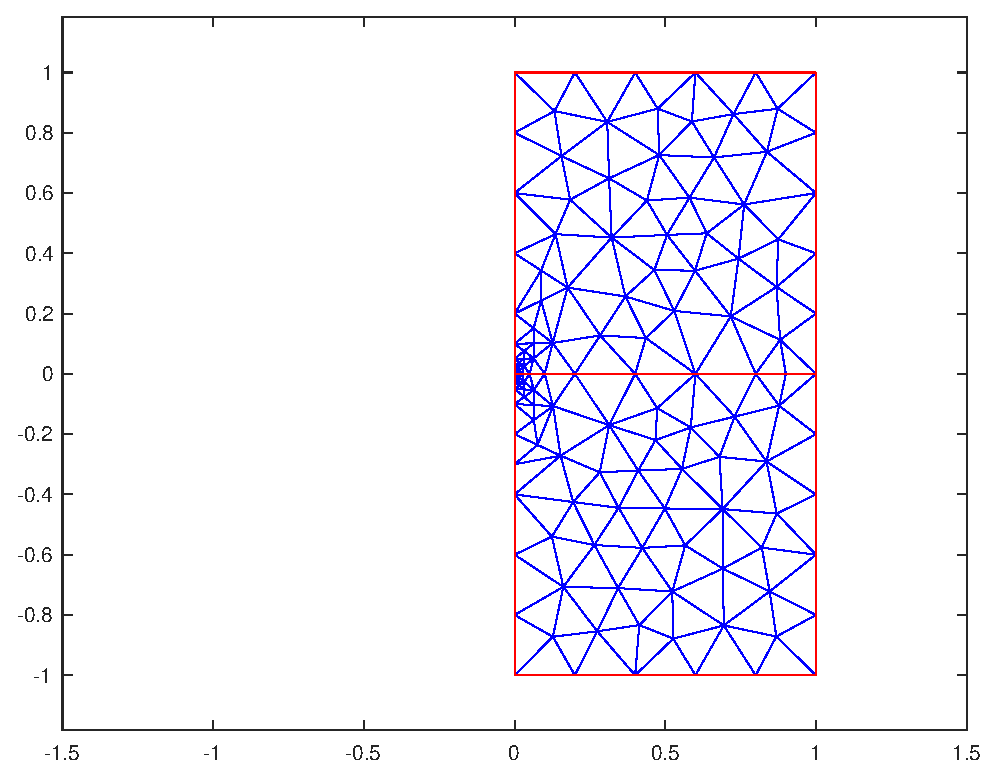
\includegraphics [width=4in]{lshape_neumann_meshsize2_01.eps}

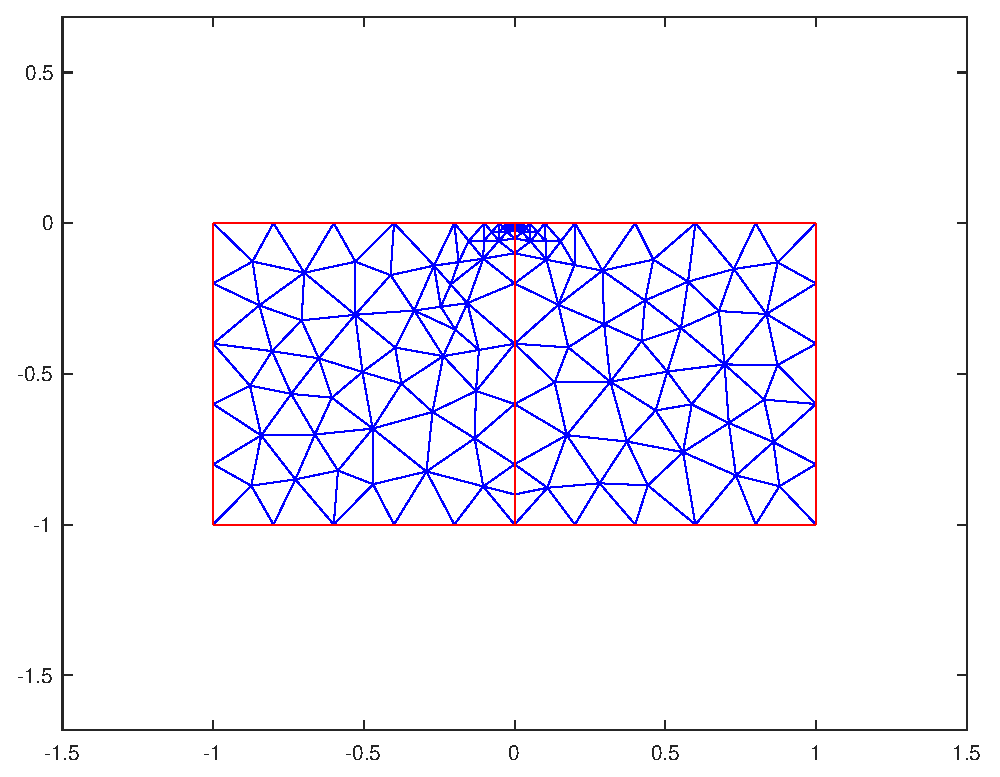
\includegraphics [width=4in]{lshape_neumann_meshsize2_02.eps}

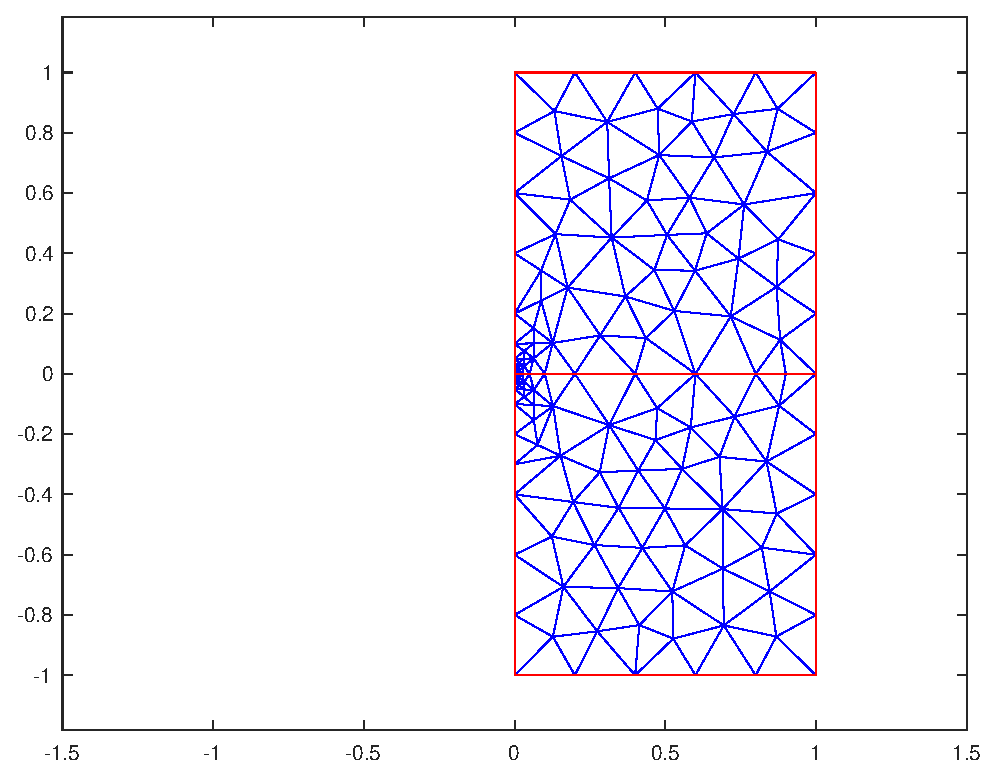
\includegraphics [width=4in]{lshape_neumann_meshsize2_04.eps}

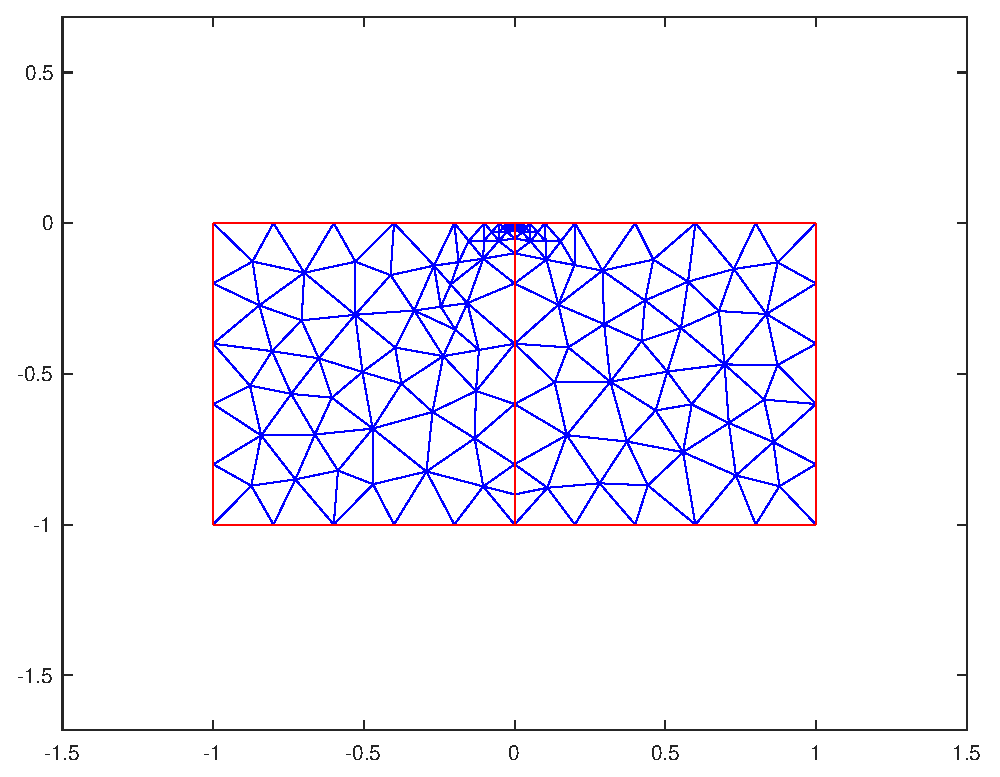
\includegraphics [width=4in]{lshape_neumann_meshsize2_05.eps}

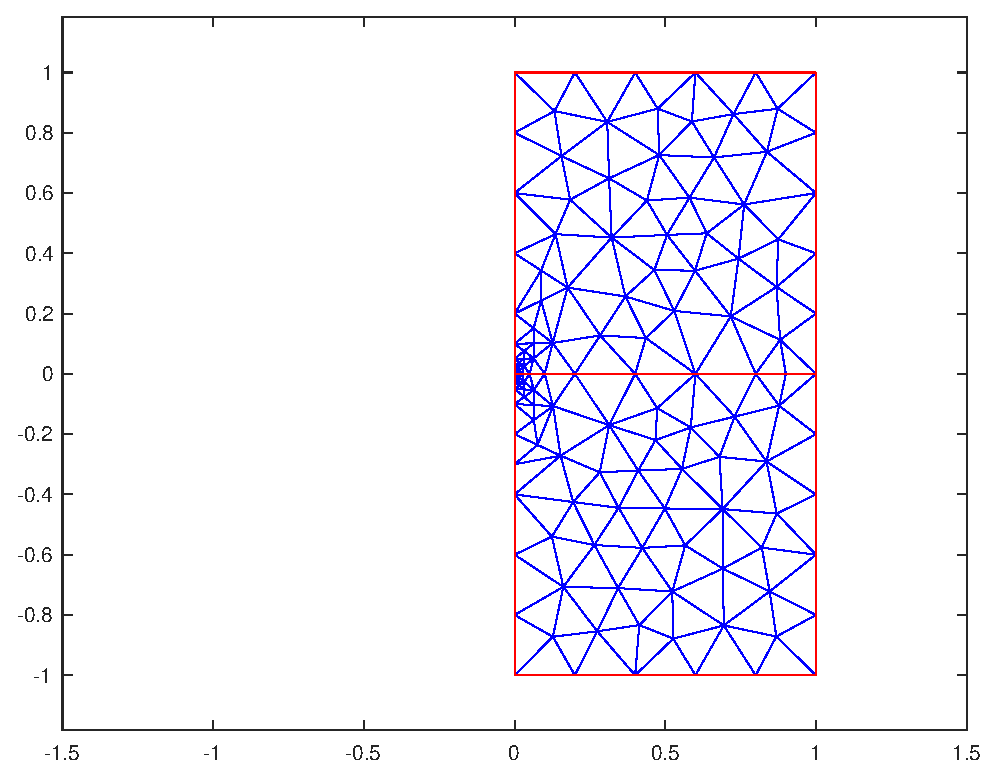
\includegraphics [width=4in]{lshape_neumann_meshsize2_07.eps}

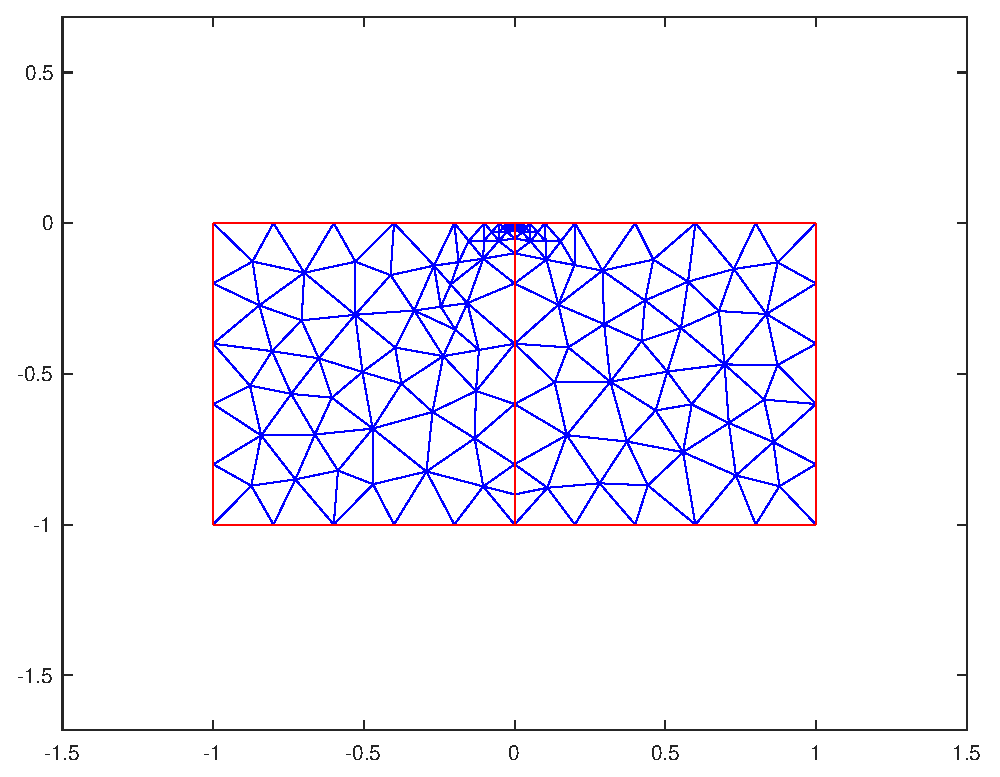
\includegraphics [width=4in]{lshape_neumann_meshsize2_08.eps}

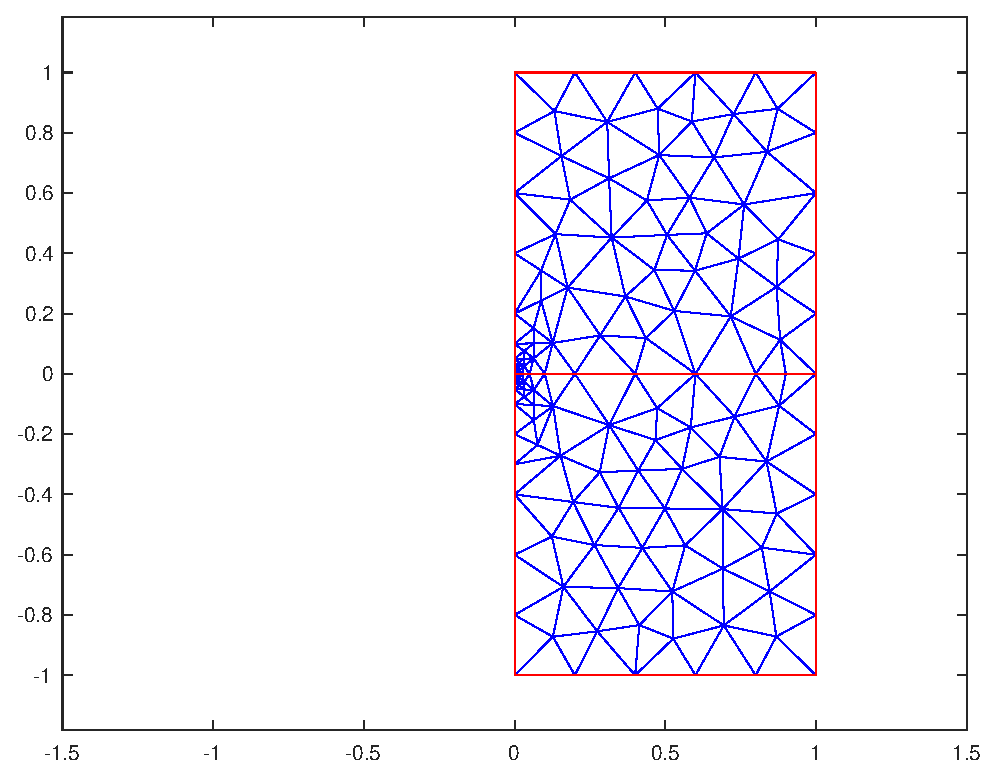
\includegraphics [width=4in]{lshape_neumann_meshsize2_10.eps}

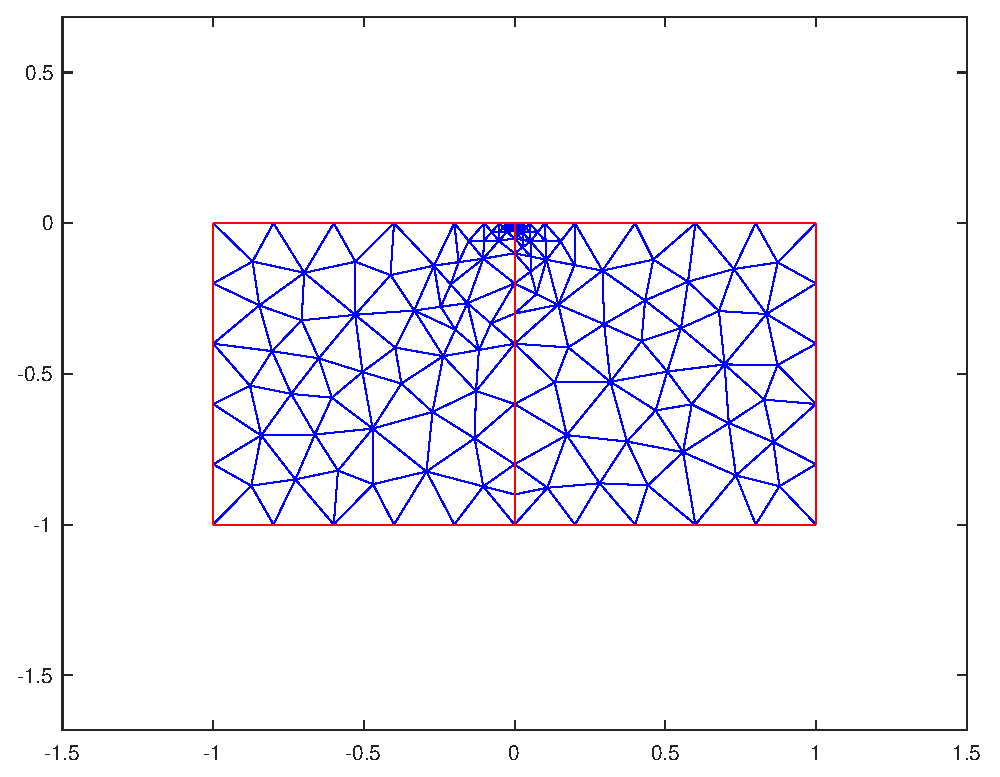
\includegraphics [width=4in]{lshape_neumann_meshsize2_11.eps}


\subsection*{Obtain relative matrices}

\begin{verbatim}
[K_up,M_up,F_up,Q_up,G_up,H_up,R_up]=assempde(b_up,p_up,e_up,t_up,c,a,f);
[K_lo,M_lo,F_lo,Q_lo,G_lo,H_lo,R_lo]=assempde(b_lo,p_lo,e_lo,t_lo,c,a,f);
\end{verbatim}


\subsection*{Assign true solution}

\begin{verbatim}
u_up_true = ones(1,length(p_up));
u_lo_true = ones(1,length(p_lo));
\end{verbatim}


\subsection*{Iterations}

\begin{verbatim}
counter = 0;
if rec == 1
    Vid = VideoWriter('Temp_video', 'MPEG-4');
    Vid.FrameRate = 3;
    Vid.Quality = 100;
    open(Vid);
end
ZZ(XX>=0) = initguess(XX(XX>=0),YY(XX>=0));
ZZ(YY<=0) = initguess(XX(YY<=0),YY(YY<=0));
figure(3);
my_plot_new(XX,YY,ZZ,az,el,v, plot_range, col_range,0,fix_axes);

if rec == 1
    frame = getframe(gcf);
    writeVideo(Vid,frame);
end
pause

% Note that pind_up2 represents the indices of the mesh points at the boundary in the
% upper domain
[pind_up1,pind_up2]=find(H_up);
% Remove the problematic point
ind=find((abs(p_up(1,pind_up2) -0)<1e-10) & (abs(p_up(2,pind_up2) -0)<1e-10));
pind_up1(ind)=[];
pind_up2(ind)=[];
% Update the Dirichlet condition matrix H_up
H_up=H_up(pind_up1,:);


[pind_lo1,pind_lo2]=find(H_lo);
% Remove the problematic point
ind=find((abs(p_lo(1,pind_lo2) -0)<1e-10) & (abs(p_lo(2,pind_lo2) -0)<1e-10));
pind_lo1(ind)=[];
pind_lo2(ind)=[];
% Update the Dirichlet condition matrix H_lo
H_lo=H_lo(pind_lo1,:);


bnew_up=zeros(length(pind_up2),1);
bnew_lo=zeros(length(pind_lo2),1);

for step = 1:Nsteps;
    if step == 1
        bfun_up = @(x,y) initguess(x,y);
    else
        bfun_up = @(x,y) tri2grid(p_lo,t_lo,u_lo,x,y);
    end
% Update  boundary conditions
for i=1:length(pind_up2);
    bnew_up(i)=bfun_up(p_up(1,pind_up2(i)),p_up(2,pind_up2(i)));
end
% Update the Dirichlet condtion vector R_up
 R_up = H_up(:,pind_up2)*bnew_up;

% Solve the pde in the upper domain
u_up=assempde(K_up,M_up,F_up,Q_up,G_up,H_up,R_up);

% Plot the solution
ZZ(XX>=0) = tri2grid(p_up,t_up,u_up,xg(indx_up),yg(indy_up));
figure(3);
my_plot_new(XX,YY,ZZ,az,el,v, plot_range, col_range, counter,fix_axes);

if rec == 1
    frame = getframe(gcf);
    writeVideo(Vid,frame);
end

pause(T)
counter = counter+1;

bfun_lo = @(x,y) tri2grid(p_up,t_up,u_up,x,y);

% Update the boundary conditions
for i=1:length(pind_lo2);
    bnew_lo(i)=bfun_lo(p_lo(1,pind_lo2(i)),p_lo(2,pind_lo2(i)));
end

% Update the Dirichlet condition vector
R_lo = H_lo(:,pind_lo2)*bnew_lo;

% Solve the pde in the lower domain
u_lo=assempde(K_lo,M_lo,F_lo,Q_lo,G_lo,H_lo,R_lo);

%Plot the solution
ZZ(YY<=0) = tri2grid(p_lo,t_lo,u_lo,xg(indx_lo),yg(indy_lo));
figure(3)
my_plot_new(XX,YY,ZZ,az,el, v, plot_range, col_range, counter,fix_axes);

if rec == 1
    frame = getframe(gcf);
    writeVideo(Vid,frame);
end

pause(T)

counter = counter+1;

% The error calculated with respect to infinity norm
errvals_inf(Nmesh/25,step)=max(max(abs([u_up(:); u_lo(:)]-[u_up_true(:); u_lo_true(:)])));

% The error calculated with respect to H1 norm

% The difference between the solution from ASM and the true solution
u_diff=ZZ-ones(size(ZZ));
% Square the difference
u_diff_square=u_diff.*u_diff;
%  stepsize on x-axis
dx=(1-(-1))/(Nplot-1);
% stepsize on y-axis
dy=(1-(-1))/(Nplot-1);
integral_1=sum(sum (dx*dy*u_diff_square(indices_all)));

% Approximate the derivatives by Central Difference Method
Du_dy=(ZZ(3:Nplot,:)-ZZ(1:Nplot-2,:))/(2*dy);
Du_dx=(ZZ(:,3:Nplot)-ZZ(:,1:Nplot-2))/(2*dx);
% Integrate on the y-direction
integrand_y=Du_dy.*Du_dy*dx*dy;
% Integrate on the x-direction
integrand_x=Du_dx.*Du_dx*dx*dy;
integrals=[integral_1,sum(sum(integrand_y(diffy_ind))),sum(sum(integrand_x(diffx_ind)))];
errvals_H1(Nmesh/25,step)=sqrt(sum(integrals));
end
\end{verbatim}

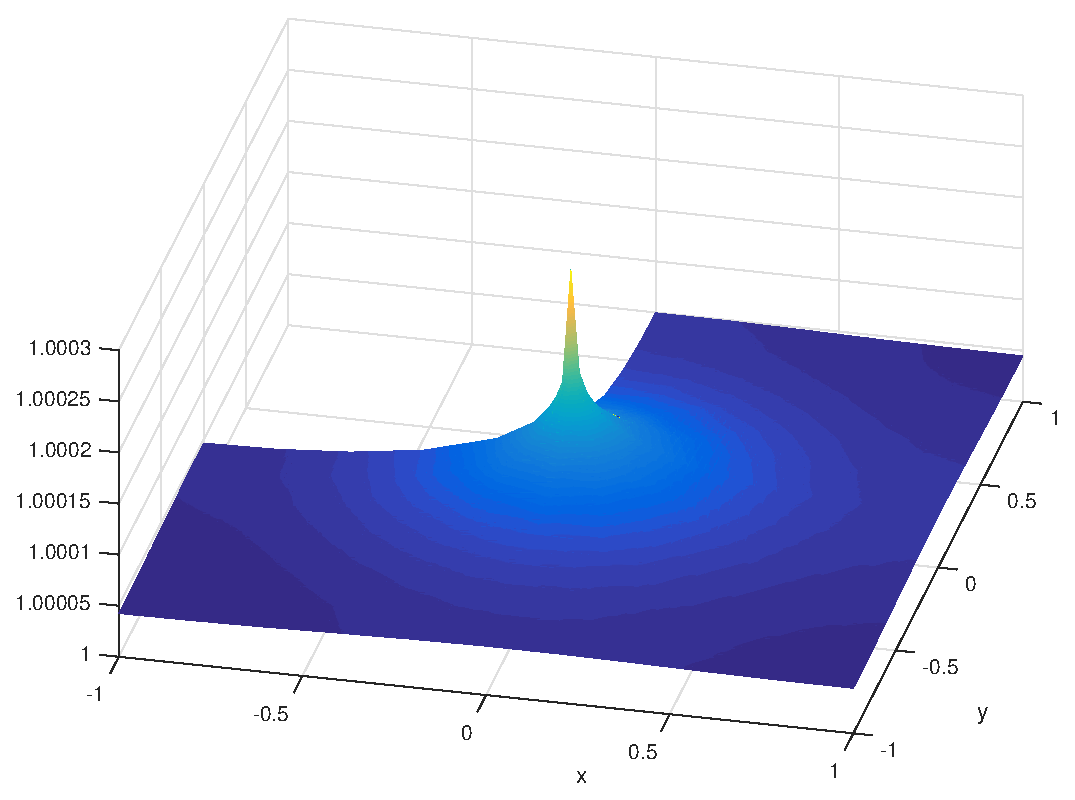
\includegraphics [width=4in]{lshape_neumann_meshsize2_03.eps}

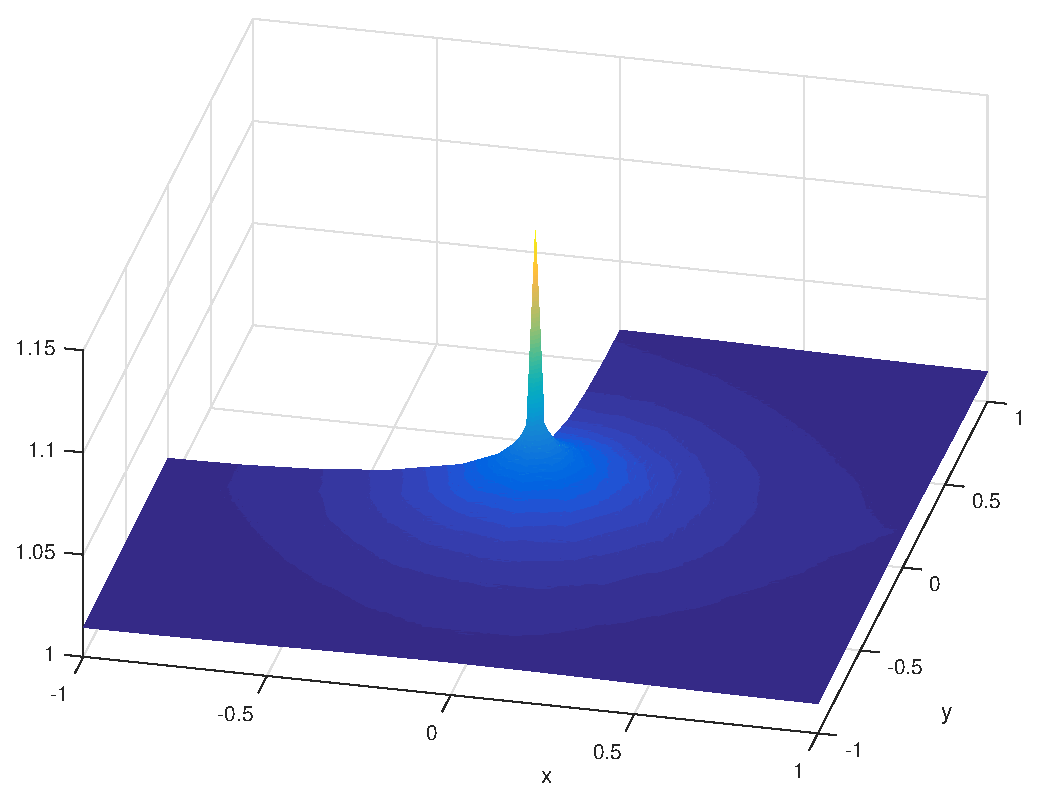
\includegraphics [width=4in]{lshape_neumann_meshsize2_06.eps}

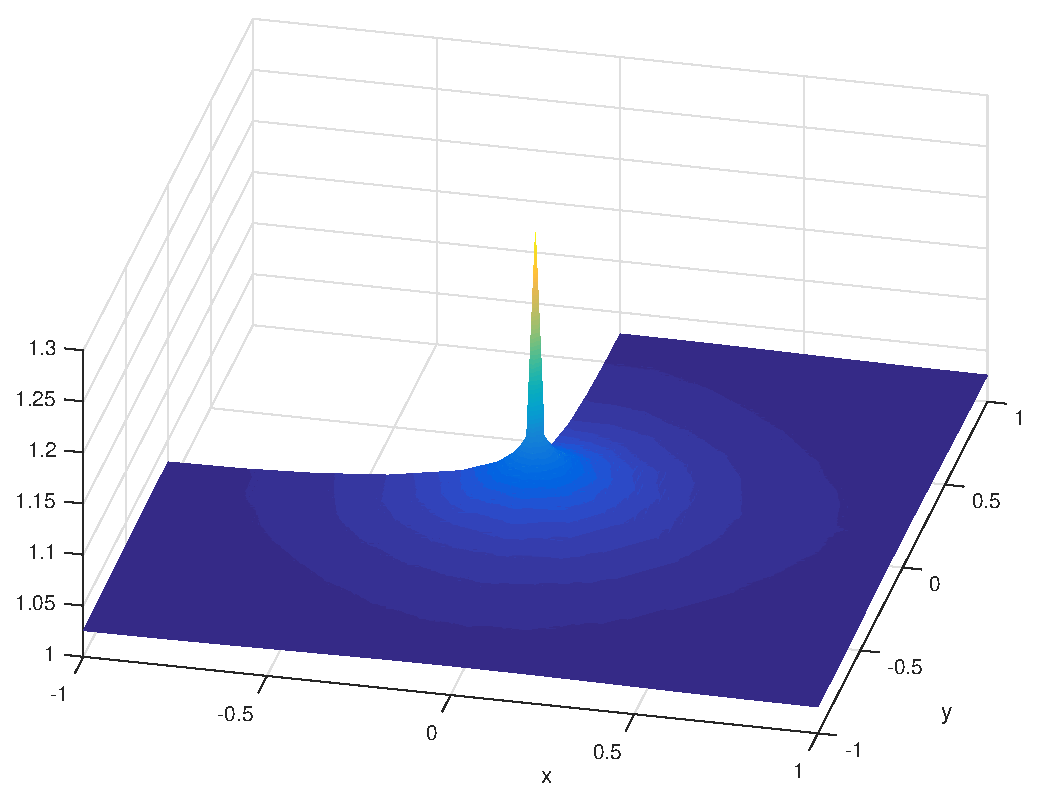
\includegraphics [width=4in]{lshape_neumann_meshsize2_09.eps}

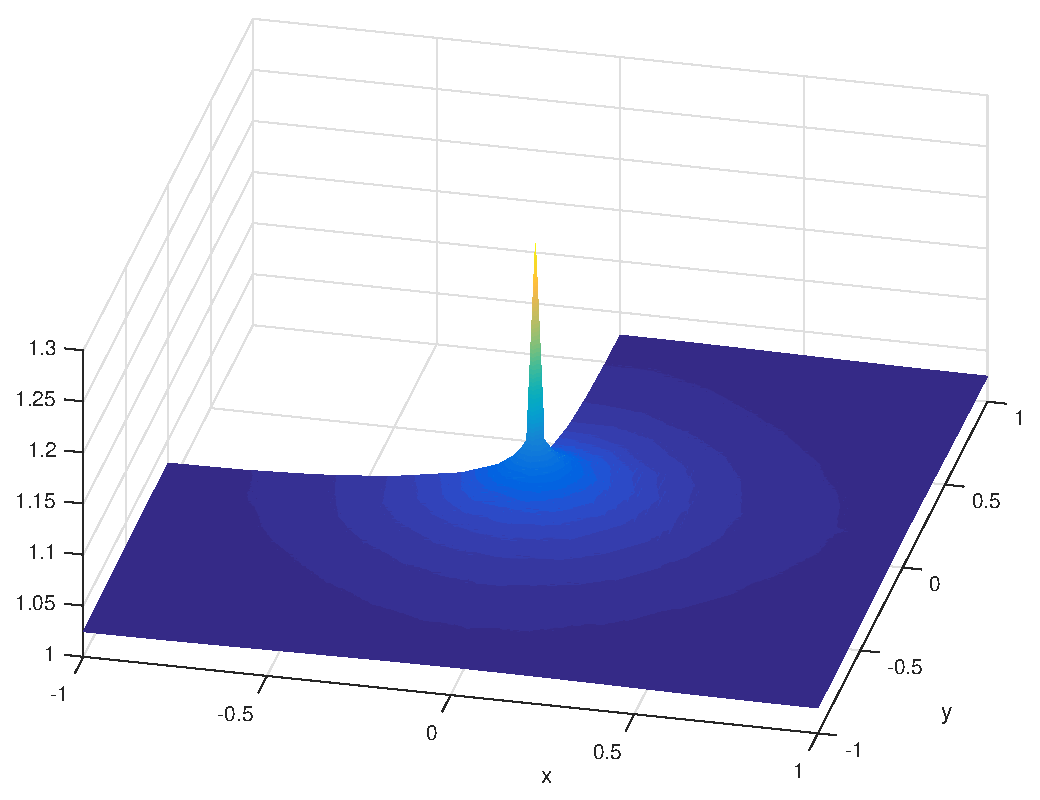
\includegraphics [width=4in]{lshape_neumann_meshsize2_12.eps}
\begin{verbatim}
end

if rec == 1
    close(Vid);
end
\end{verbatim}


\subsection*{Plot of \texttt{\ensuremath{|}u\_n-u\_true}\ensuremath{|} versus Nsteps}

\begin{verbatim}
figure(4)
nn = 1:Nsteps;
semilogy(nn,[errvals_inf(1,:);errvals_inf(2,:);errvals_inf(3,:);errvals_inf(4,:)]);
legend('Nmesh=25','Nmesh=50', 'Nmesh=75','Nmesh=100')
xlabel('Number of Iterations'); % x-axis label
ylabel('Log(errvals_{inf})') ;    % y-axis label

figure(5)
nn = 1:Nsteps;
semilogy(nn,[errvals_H1(1,:);errvals_H1(2,:);errvals_H1(3,:);errvals_H1(4,:)]);
legend('Nmesh=25','Nmesh=50', 'Nmesh=75','Nmesh=100');
xlabel('Number of Iterations'); % x-axis label
ylabel('Log(errvals_{H1})');     % y-axis label
toc
\end{verbatim}

        \color{lightgray} \begin{verbatim}Elapsed time is 90.622654 seconds.
\end{verbatim} \color{black}
    
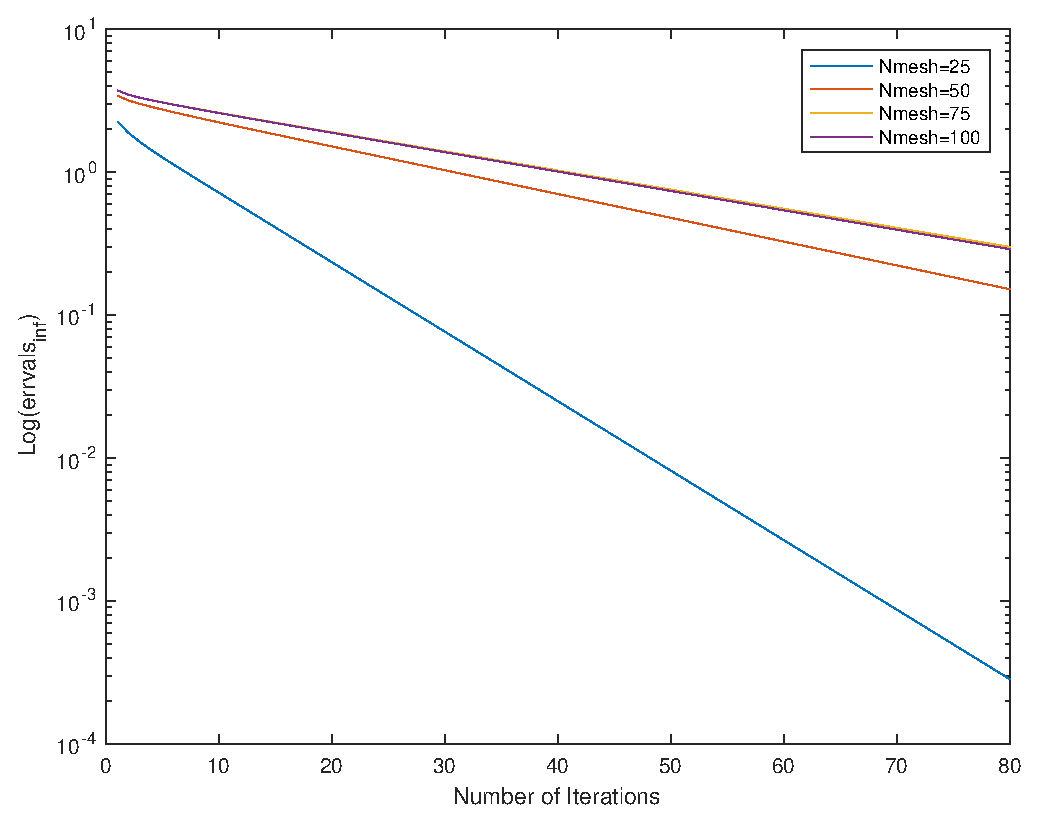
\includegraphics [width=4in]{lshape_neumann_meshsize2_13.eps}

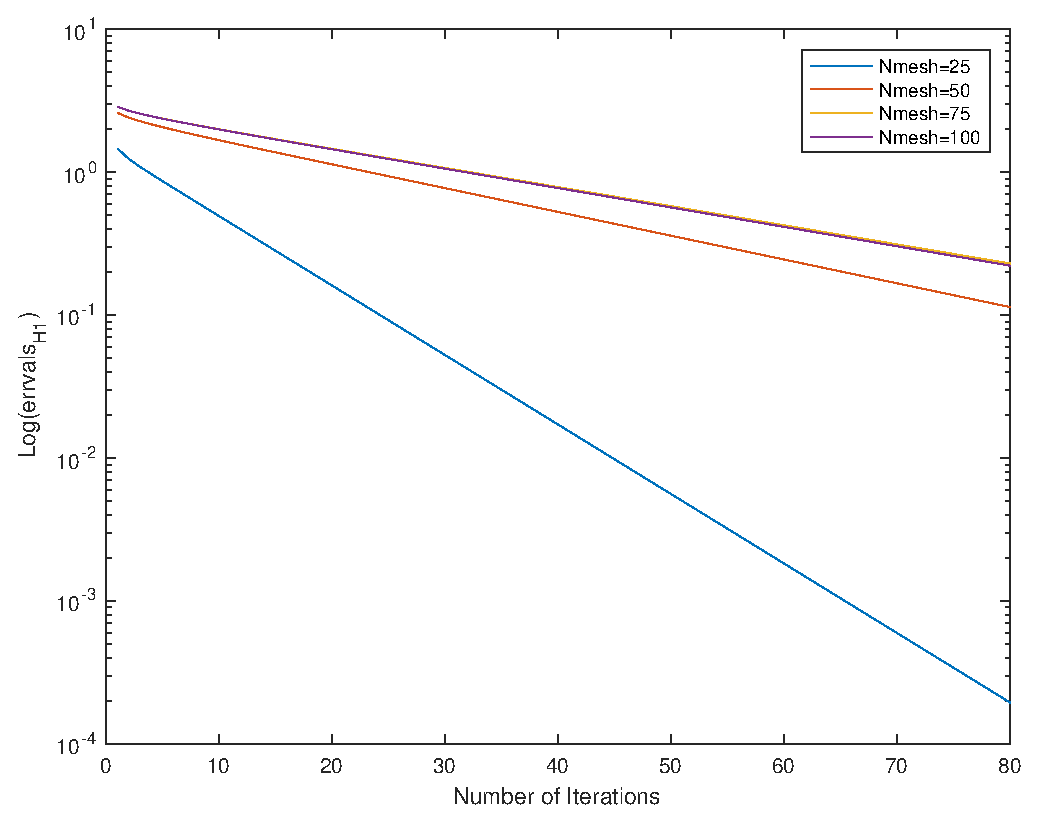
\includegraphics [width=4in]{lshape_neumann_meshsize2_14.eps}

